% !TEX root = ../../../main.tex

\toggletrue{image}
\toggletrue{imagehover}
\chapterimage{protocol_2x}
\chapterimagetitle{\uppercase{Protocol}}
\chapterimageurl{https://xkcd.com/1323/}
\chapterimagehover{Changing the names would be easier, but if you're not comfortable lying, try only making friends with people named Alice, Bob, Carol, etc.}

% TODO add to bib: RSA and public-key cryptography / Richard A. Mollin. p. cm. — (Discrete mathematics and its applicatoins) Includes bibliographical references and index. ISBN 1-58488-338-3

\chapter{Grundlagen}
\label{chapter-schluesselfestlegungsprotokolle-grundlagen}

Alle bisherigen Kryptosysteme wurden unter der Annahme betrachtet, dass Alice und Bob einen \textbf{gemeinsamen} Schlüssel besitzen. Dieser Schlüssel wurde von Alice zur Verschlüsselung und von Bob zur Entschlüsselung (symmetrisches Kryptosystem) benutzt. In diesem Teil klären wir nun, wie Alice und Bob überhaupt zu einem gemeinsamen Schlüssel kommen. Zuvor klären wir die wichtigsten Begriffe. Die Lernziele lauten:

\newcommand{\grundlagenSchluesselfestlegungsprotokolleLernziele}{
\protect\begin{todolist}
\item Sie definieren die Begriffe Kommunikation, Protokoll und Schlüsselfestlegungsprotokoll.
\item Sie definieren die Begriffe Schlüsselverteilung und Schlüsselvereinbarung.
\item Sie erklären den Unterschied zwischen der Schlüsselverteilung und Schlüsselvereinbarung.
\end{todolist}
}

\lernziel{\autoref{chapter-schluesselfestlegungsprotokolle-grundlagen}, \nameref{chapter-schluesselfestlegungsprotokolle-grundlagen}}{\protect\grundlagenSchluesselfestlegungsprotokolleLernziele}

\grundlagenSchluesselfestlegungsprotokolleLernziele

\begin{definition}[Kommunikation und Protokoll]
Unter \textbf{Kommunikation} verstehen wir den Austausch von Informationen zwischen zwei oder mehr Kommunikationspartnern. Ein \textbf{Protokoll} definiert sowohl den zeitlichen Ablauf der Kommunikation als auch Form und Inhalt der jeweils übermittelten Informationen \cite{datzko2023informatiksek2}.
\end{definition}

\begin{figure}[htb]
\centering
\begin{minipage}{0.55\textwidth}
\autoref{figure-protocol} zeigt die Idee eines Protokolls an einem Beispiel aus dem Alltag. In der Informatik wird ein Protokoll typischerweise durch ein Programm realisiert. Computerprogramme kommunizieren dann gemäss Protokollen, um Daten auszutauschen.
Ein \textbf{Schlüsselfestlegungsprotokoll} (eng. key establishment protocols) ist ein kryptographisches Protokoll, welches zwischen zwei Parteien einen gemeinsamen Schlüssel für ein symmetrisches Kryptosystem festlegt. Wir können dieses Ziel auf zwei Methoden erreichen.
\end{minipage}
\hfill
\begin{minipage}{0.4\textwidth}
\centering
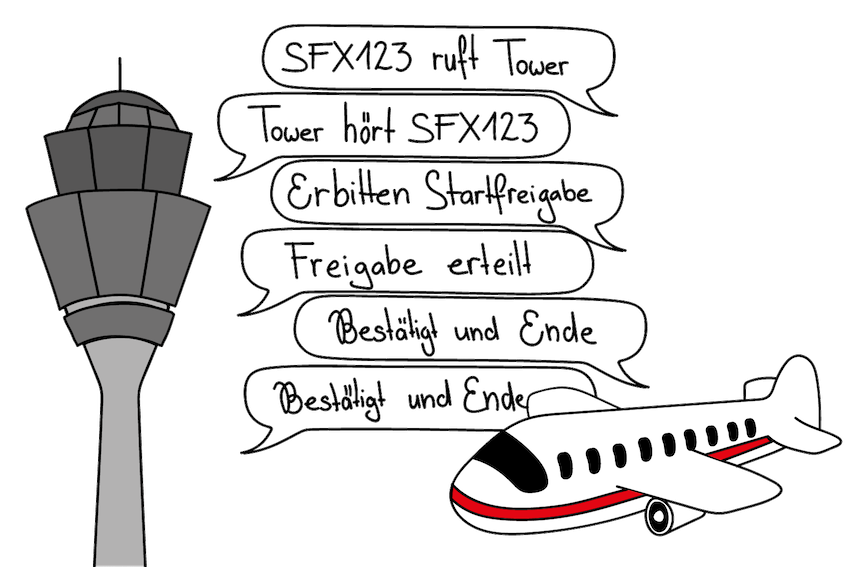
\includegraphics[scale=0.15]{protokoll}
\caption{Protokollbeispiel bei der Kommunikation zwischen Flughafen und Flugzeug \cite{hohl2023protokoll}.}
\label{figure-protocol}
\end{minipage}
\end{figure}

\begin{definition}[Schlüsselverteilung (eng. key distribution)]
Alice \textbf{bestimmt} einen gemeinsamen Schlüssel und teilt den Schlüssel dann auf sicherem Weg Bob mit.
\end{definition}

\begin{definition}[Schlüsselvereinbarung (eng. key agreement)]
Alice und Bob agieren \textbf{gemeinsam} und \textbf{erzeugen zusammen} einen gemeinsamen Schlüssel. Beide Parteien sind gleichberechtigt.
\end{definition}

Wir schauen uns in den folgenden Kapiteln beide Methoden an.